%%%%%%%%%%%%%%%%%%%%%%%%%%%%%%%%%%%%%%%%%%%%%%%%%%%%%%%%%%%%%%%%%%%%%%%%
\chapter{Introduction}\label{chap:intro}
The long-standing challenge for research in computer science is the understanding of written text and extraction of useful information from it. Text that is created by humans is often unstructured and ambiguous, whereas machine learning algorithms prefer well-defined fixed-length inputs and outputs. Therefore, machine learning algorithms cannot work with raw text directly and the text has to be converted into vectors of features.
\\
\noindent
Traditional \emph{Natural Language Processing} (NLP) systems treat words as atomic units. Regarding vectors, each word would be treated as a one-hot vector the size of the vocabulary. These vectors are sparse and orthogonal, and therefore contain no notion of similarity among themselves. For example, if a user is searching for \emph{``Heidelberg Hotel''}, documents containing \emph{``Heidelberg Motel''} will be disregard since the dot product of the one-hot vectors of \emph{``Hotel''} and \emph{``Motel''} is zero. On the other hand, distributed vector space models represent words in a continuous vector space, where a word is represented by its neighbors' means. These models are based on the idea that similar words tend to happen in a similar context or as the British linguist, J.R. Firth, said:
\\
\\
\noindent
\say{You shall know a word by the company it keeps.} (J.R. Firth 1957)\\
\\
\noindent
These distributed representations try to map words to a dense vector, such that words with closer meanings are mapped to the nearby points and the similarity between them can be computed based on their distance in space.
\\
\noindent 
Learning dense vector representations of words was introduced by the pioneering paper by~\brackettext{\cite{Bengio:2003:NPL:944919.944966}}, in which a feature vector, much smaller than the size of the vocabulary, was used to express words using a probabilistic model. The work of~\brackettext{\cite{Collobert:2011:NLP:1953048.2078186}} proved that word representation could not only be achieved through probabilistic models, but that neural network architectures can also learn these internal representations from vast amounts of mostly unlabeled training data.
\\
\noindent
The first simple and scalable model to learn such embeddings is \emph{word2vec} presented by \brackettext{\cite{DBLP:journals/corr/abs-1301-3781}}, where the aim is to capture the meaning of a word based on the surrounding context. The goal of the model is, given a center word, to predict the words that occur in its surroundings. word2vec uses a shallow neural network with one hidden layer to process non-labeled documents. The neural network architecture contains two models, \emph{continuous bag-of-words} (CBOW) and the \emph{skip-gram} architecture. Both are shown in Figure~\ref{fig:skip_gram}. The CBOW architecture predicts the current word based on the context and the skip-gram predicts surrounding words given the current word.
\begin{figure}
\centering

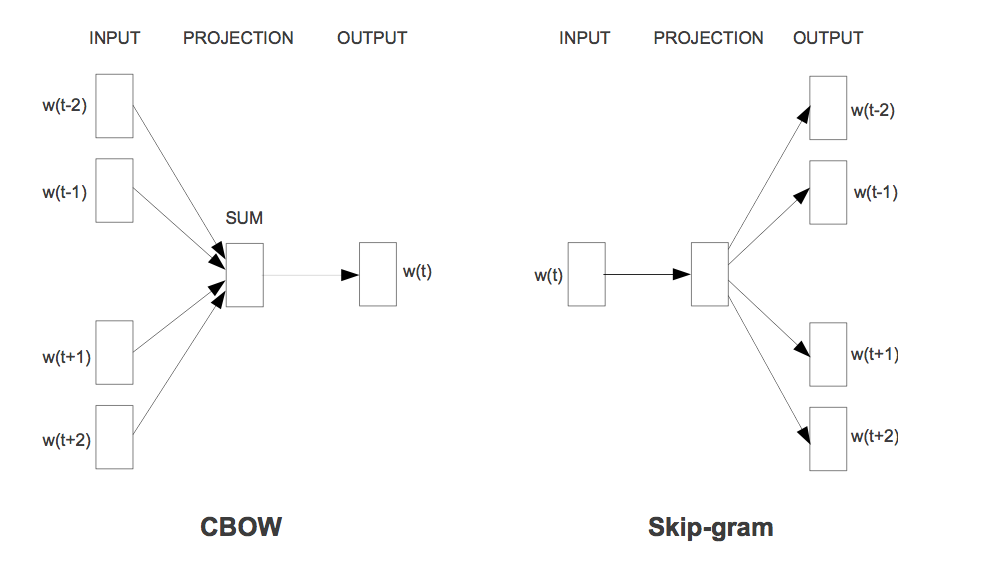
\includegraphics[width=0.7\linewidth , height=0.5\linewidth]{images/CBOW_SkipGram.png}
\caption{Predict a word, given the preceding and following words (Continuous Bag of Words, CBOW) and predict the preceding and following words, given a word (Skip-Gram). Image from \brackettext{\cite{DBLP:journals/corr/abs-1301-3781}}.}
\label{fig:skip_gram}
\end{figure}
If sufficient data is used for training, word2vec can predict with high accuracy the word's meaning based on its surrounding words in the corpus and also successfully capture semantic relations, such as country and capital relations, as well as syntactic relations. For example, present tense and past tense, or even meaningful algebraic operations are supported. For example vector of  \emph{``man''} twill have approximately the same distance to  \emph{``brother''} as \emph{``women''} to \emph{``sister''}: $V_{brother}-  V_{man} +V_{women} \approx V_{sister}$. There exists numerous variation of this model, from taking the character level information into account (fasttext)~\brackettext{\cite{DBLP:journals/corr/BojanowskiGJM16}} to incorporating the statistics of the whole corpus (GloVe model)~\brackettext{\cite{DBLP:conf/emnlp/PenningtonSM14}}. GloVe model in particular speeds up the learning and when trained on a large corpus tends to generate more promising results on downstream tasks such as named entity recognition.\\
word2vec based methods, although good at capturing semantics, have some drawbacks. They treat each word equally regardless of their type (e.g., person or location). One valuable tool in NLP that takes this information into account is implicit networks of entities extracted from unstructured text as demonstrated in the work of~\brackettext{\cite{Rousseau:2013:GTN:2505515.2505671}}. These networks, similar to knowledge graphs, encode relationships between entities but unlike them, information of the type of connection is unknown. On the other hand, the strength of relationships can be inferred from edge weights. \emph{LOAD} ~\brackettext{\cite{Spitz2016a}} is an implicit entity network, in which the statistics of a corpus of text is encoded in the edge weights between entities of type actor, location, organisation, date, and term. With LOAD, similar to word2vec, many relations between nearby words can be extracted. Moreover, the type-specific nature of the network allows for more flexibility and encodes more information than mere neighborhood structure.

 \section{How to Interpret Word Embeddings? }

Dense vector representations of words can encode underlying complexity and latent trends in the data, but they are far from being interpretable. In many cases, the semantic structure is heterogeneously distributed across the embedding dimensions, which makes interpretation challenging. 
Recently, some work have been done to make the embedding less ambiguous. In the work of \brackettext{\cite{DBLP:journals/corr/FaruquiTYDS15}} transformation of word vectors into sparse (and optionally binary) vectors was proposed. Each vector is projected into an over-complete binary vector, where each dimension represents a feature similiar to ones used in traditional NLP systems but found automatically during training. $0$ or $1$ indicates the presents or abscence of a certain feature. However, since their dimensions are binary valued, there is no notion of the extent to which a word participates in a particular dimension. Rotating the word vectors was introduced by \brackettext{\cite{prak2017}} to improve the interpretability.  \brackettext{\cite{DBLP:journals/corr/abs-1711-08792}} proposes a neural network-based approach to the problem by using sparse Auto-encoders. 
Nevertheless, both of these methods are applied as a later processing step to the trained embedding and offer no solution to learn the embeddings as an interpretable component during training time. Moreover, the meaning of a specific dimension has been investigated based on the words that most activate it. It is still unknown, if the model predicts \emph{``London"} and \emph{``Berlin"} as similar, whether they both appeared in same the context location-wise, e.g., whether both are capitals and are situated in Europe or because they share the same organizations, e.g., many companies moved their offices from London to Berlin after the Brexit. This information can in some extent be extracted from networks such as LOAD, where the entity type is specified for each node.\\
In the following, we propose a method to combine the benefits of name entity graphs with word vectors to generate more interpretable word embeddings.

\section{Objective and Contributions}

In this study, we introduce facetted embedding as a method to better understand the semantic structures and increase the interpretability of vector space models. Facetted embedding is a vector space model, in which each part of the vector represents different properties of the word, namely  locations, actors or organisations associated with it, dates of its mention and terms that define its meaning. One visual example of such an embedding ($V$) is shown below: \\
\mathleft
\begin{equation}
V=\left[ \underbrace { \begin{matrix}{ a }_{ 1,1 } ... { a }_{ 1,M } \end{matrix} } |\underbrace { \begin{matrix}{ a }_{ 1,M+1 } ... { a }_{ 1,2M } \end{matrix} } |\underbrace { \begin{matrix}{ a }_{ 1,2M+1 } ... { a }_{ 1,3M } \end{matrix} } |\underbrace { \begin{matrix}{ a }_{ 1,3M+1 } ... { a }_{ 1,4M } \end{matrix} } |\underbrace { \begin{matrix}{ a }_{ 14M+1 } ... { a }_{ 1,5M } \end{matrix} }  \right] 
\label{eq:concat_vec}
\end{equation}
$$ \quad  ACT \quad  \qquad  LOC\qquad \qquad ORG\qquad \quad \qquad DAT\qquad \quad  \qquad  TER\qquad \qquad$$
\mathcenter
\\
The type-information of an entity is encoded in a named entity graph. Hence, it is reasonable that this graph will be used as an input instead of the raw textual corpus. The facetted embedding takes as input the edge weights of the LOAD network along with the type information and generates a separate embedding structure for each word based on the surrounding entities. In contrast to simple word2vec, each part of the embedding vector is responsible for encoding one of the five entity types available by LOAD, e.g., the actors part only encodes the actors in the context of a word.\\
The advantage of this approach is that the similarity of the words can now be broken down into their different attributes. If two entities are closer in location space and further in actors space, it is possible that they are situated close locally, but are not related to the same people. These embedding will be a useful tool to explore and understand changes in news streams. Exploring and visualizing different dimensions of an embedding over time will give us insight into how that entity has evolved. For example, it is expected that since \emph{``Donald Trump"} has become president, the location dimension of his embedding changes dramatically as he has moved to White House and travels more often. The organisations, however, tend to stay relatively stable as his business did not undergo dramatic changes. Without the separation of dimensions, it is hard to identify in which particular aspect has the entity most transformed. In addition, since dimensions are independent and can be analysed separately, the similarity between two entities becomes more interpretable. It would be possible to identify if two similar entities are mentioned in the same locations or in the context of related actors. \\
Separate dimensions also provide flexibility in information retrieval tasks. Facetted embeddings encode the type of the entities surrounding a word. This type-specific information can be used in the search, where one can query for entities that are closer to a certain word in the temporal or location aspect. The normal embedding treats all the word equally and therefore, can not reflect this type of similarity. Since the dimensions are independent and can be combined in an arbitrary way, a combination of different dimensions can tailor the search results further and create a type-specific search. \\
Recent work in entity disambiguation uses pre-trained word embedding in combination with the recurrent neural network to enhance the accuracy of the system~\brackettext{\cite{DBLP:journals/corr/LampleBSKD16}}. Since the facetted embedding encodes additional type information in comparison to normal embedding, these embedding can potentially enhance these models. For example, to \emph{``Washington"} as a political person tends to appear more often with the same actors and has different actor dimension than \emph{``Washington DC"} as a location. Additionally, since the facetted embedding are learned on the already disambiguated entities (from LOAD network), the embedding of \emph{``Washington"} as a state and as a politician are different from each other, whereas in general word embeddings this distinction cannot be made. \\
Training word embedding for a specific task such as the analysis of news articles is by no means a novel task. Word embeddings have been tailored to for dependency parsing (analysis of the grammatical structure of a sentence and establishing relationships between words)~\brackettext{\cite{P14-2131}} and semantic relation classification \brackettext{\cite{DBLP:journals/corr/HashimotoSMT15}.} But none of the methods create separate interpretable dimensions and their usage is mostly limited to the tasked they are trained for. In this thesis we aim to introduce facetted embedding as a general framework for learning embeddings with separable dimensions, where their usage is not limited to only to the analysis of news articles but can be trained on any corpus can be tailored further to match a specific downstream task. 
\section{Overview}

The remainder of this thesis is structured as follows: In Chapter~\ref{chap:background}, the background information required for the model and related work is discussed, with a brief introduction to basics of NLP and neural networks. The GloVe model is the base of facetted embedding and therefore, is explained in more detail in this chapter as a pre-requisite for understanding how the final model works. Chapter~\ref{chap:main} contains an in-depth definition of the facetted embeddings, how they are generated, different parameters and the cost function. The \ref{chap:eval}th chapter contains the test cases and evaluation results. The model is analysed using visualization and also tested against well-known analogy and word similarity datasets. The work is closed with a conclusion and outlook on possible future work in Chapter~\ref{chap:concl}. 
